%%%%%%%%%%%%%%%%%%%%%%%%%%%%%%%%%%%%%%%%%
% Beamer Presentation
% LaTeX Template
% Version 1.0 (10/11/12)
%
% This template has been downloaded from:
% http://www.LaTeXTemplates.com
%
% License:
% CC BY-NC-SA 3.0 (http://creativecommons.org/licenses/by-nc-sa/3.0/)
%
%%%%%%%%%%%%%%%%%%%%%%%%%%%%%%%%%%%%%%%%%

%----------------------------------------------------------------------------------------
%	PACKAGES AND THEMES
%----------------------------------------------------------------------------------------

\documentclass{beamer}

\mode<presentation> {

% The Beamer class comes with a number of default slide themes
% which change the colors and layouts of slides. Below this is a list
% of all the themes, uncomment each in turn to see what they look like.

%\usetheme{default}
%\usetheme{AnnArbor}
%\usetheme{Antibes}
%\usetheme{Bergen}
%\usetheme{Berkeley}
%\usetheme{Berlin}
%\usetheme{Boadilla}
\usetheme{CambridgeUS}
%\usetheme{Copenhagen}
%\usetheme{Darmstadt}
%\usetheme{Dresden}
%\usetheme{Frankfurt}
%\usetheme{Goettingen}
%\usetheme{Hannover}
%\usetheme{Ilmenau}
%\usetheme{JuanLesPins}
%\usetheme{Luebeck}
%\usetheme{Madrid}
%\usetheme{Malmoe}
%\usetheme{Marburg}
%\usetheme{Montpellier}
%\usetheme{PaloAlto}
%\usetheme{Pittsburgh}
%\usetheme{Rochester}
%\usetheme{Singapore}
%\usetheme{Szeged}
%\usetheme{Warsaw}
% As well as themes, the Beamer class has a number of color themes
% for any slide theme. Uncomment each of these in turn to see how it
% changes the colors of your current slide theme.

%\usecolortheme{albatross}
\usecolortheme{beaver}
%\usecolortheme{beetle}
%\usecolortheme{crane}
%\usecolortheme{dolphin}
%\usecolortheme{dove}
%\usecolortheme{fly}
%\usecolortheme{lily}
%\usecolortheme{orchid}
%\usecolortheme{rose}
%\usecolortheme{seagull}
%\usecolortheme{seahorse}
%\usecolortheme{whale}
%\usecolortheme{wolverine}

%\setbeamertemplate{footline} % To remove the footer line in all slides uncomment this line
\setbeamertemplate{footline}[page number] % To replace the footer line in all slides with a simple slide count uncomment this line

%\setbeamertemplate{navigation symbols}{} % To remove the navigation symbols from the bottom of all slides uncomment this line
}
\usepackage{bbm}
\usepackage{tikz}
\usetikzlibrary{graphs}
\usetikzlibrary{overlay-beamer-styles}
\newcommand{\tikzmark}[1]{\tikz[remember picture] \node[coordinate] (#1) {#1};}
\usepackage{verbatim}
\usetikzlibrary{arrows,shapes}
\usepackage{graphicx} % Allows including images
\usepackage{amsmath}
\newcommand\scalemath[2]{\scalebox{#1}{\mbox{\ensuremath{\displaystyle #2}}}}
\newcommand\numberthis{\addtocounter{equation}{1}\tag{\theequation}}
\usepackage{booktabs} % Allows the use of \toprule, \midrule and \bottomrule in tables
\usepackage{hyperref}
\usepackage[font=footnotesize,justification=centering]{caption}
\tikzset{
  invisible/.style={opacity=0},
  visible on/.style={alt={#1{}{invisible}}},
  alt/.code args={<#1>#2#3}{%
    \alt<#1>{\pgfkeysalso{#2}}{\pgfkeysalso{#3}} % \pgfkeysalso doesn't change the path
  },
  marked/.style={
    %color=white,
    fill=green!20,
  },
  marked on/.style={alt=#1{marked}{}}
  }
%\usepackage{algorithm,algorithmic}
\usepackage[ruled,vlined,linesnumbered]{algorithm2e}
%----------------------------------------------------------------------------------------
%	TITLE PAGE
%----------------------------------------------------------------------------------------

\title[ADMM FPGA]{An Embedded Scalable Linear Model Predictive Hardware-based Controller using ADMM} % The short title appears at the bottom of every slide, the full title is only on the title page

\author{Pei Zhang, Joseph Zambreno and Phillip H. Jones} % Your name
\institute[ISU] % Your institution as it will appear on the bottom of every slide, may be shorthand to save space
{
\textit{Presenter: Pei Zhang}\\
\medskip
Iowa State University\\ % Your institution for the title page
\medskip

\textit{peizhang@iastate.edu} % Your email address
}
\date{\today} % Date, can be changed to a custom date



\begin{document}


\begin{frame}
\titlepage % Print the title page as the first slide
\end{frame}

\begin{frame}
\frametitle{Overview} % Table of contents slide, comment this block out to remove it
\tableofcontents % Throughout your presentation, if you choose to use \section{} and \subsection{} commands, these will automatically be printed on this slide as an overview of your presentation
\end{frame}

%----------------------------------------------------------------------------------------
%	PRESENTATION SLIDES
%----------------------------------------------------------------------------------------

\section{Related Work}
%------------------------------------------------
\begin{frame}
\frametitle{Quadratic Programming (QP) solutions}

MPC can be posed as a Quadratic Programming problem.\\~\\

QP problems can be solved reliably via various iterative methods.
\begin{itemize}
\item Interior-Point Method (IPM)
\item Active Set Method (ASM)
\item Splitting Method
\end{itemize}

\end{frame}
%------------------------------------------------

%------------------------------------------------
\begin{frame}
\frametitle{FPGA-based QP solutions}
Compare IPM and ASM in FPGA\\~\\
\begin{itemize}
\item ASM gives lower computing complexity and converges faster when the number of decision variables and constraints are small.
\item IPM is a better choice when considering scalability.
\end{itemize}
\end{frame}
%------------------------------------------------


\section{Background}
\subsection{State Space Model}
%------------------------------------------------
\begin{frame}
\frametitle{State Space Model}
A discrete state-space model defines what state a system will be in one-time step into the future:
\begin{equation}
\label{eq:xk}
x_{k+1}=A x_k + B u_k 
\end{equation}  
\begin{equation}
\label{eq:yk}
y_{k}=C x_k + D u_k  
\end{equation}  
\begin{itemize}
  \item $x_k$ represents the state of the system at time $k$
  \item $u_k$ represents the input acting on the system at time $k$
  \item $y_k$ represents outputs of the system at time $k$
  \item $A$ is a matrix that defines the internal dynamics of the system
  \item $B$ is a matrix that defines how the input acting upon the system impact its state
  \item $C$ is a matrix that transforms states of the system into outputs ($y_k$)
\end{itemize}
\end{frame}
%------------------------------------------------


\subsection{Model Predictive Optimal Control}
%------------------------------------------------

\begin{frame}
\frametitle{Augmented Vector}
\begin{equation}
\scalemath{0.8}{
U_k=
\begin{bmatrix}
u_k\\
u_{k+1}\\
\vdots \\
u_{k+H_u}
\end{bmatrix}
\text{,}\quad
\Delta U_k=
\begin{bmatrix}
\Delta u_k\\
\Delta u_{k+1}\\
\vdots \\
\Delta u_{k+H_{u-1}}
\end{bmatrix}
\text{,}\quad
X_k=
\begin{bmatrix}
x_k\\
x_{k+1}\\
\vdots \\
x_{k+H_p}
\end{bmatrix}\label{eq:aug}}
\end{equation}
Where:
\begin{itemize}
	\item $H_u$: changeable future input horizon. We assume input $u_k$ will be constant after $H_u$ time steps.
	\item $H_p$: prediction horizon. Normally, $H_p\geq H_u$. 
	\item $U_k \in \mathbb{R}^{M(H_{u}+1)}$, $\Delta U_k \in \mathbb{R}^{MH_{u}}$, $X_k \in \mathbb{R}^{N(H_{p}+1)}$.
\end{itemize}
\end{frame}
%------------------------------------------------
%------------------------------------------------
\begin{frame}
\frametitle{Cost Function}
\begin{equation}
\scalemath{0.8}{
\begin{split}
\mathbb{C}(k)=\frac{1}{2}\Big( \sum_{i=k}^{k+H_p}(x_i^Tq_ix_i-2r_i^Tq_ix_i)+\sum_{i=k}^{k+H_u}u_i^Tp_iu_i+\sum_{i=k}^{k+H_{u-1}}\Delta u_i^Ts_i\Delta u_i\Big)+Const
\label{eq:costf}
\end{split}}
\end{equation}
\begin{equation}
\scalemath{0.8}{
\mathbb{C}(k)=\frac{1}{2}
\begin{bmatrix}
X_k\\
U_k\\
\Delta U_k
\end{bmatrix}^T
\begin{bmatrix}
Q& & \\
 &P& \\
& &S 
\end{bmatrix}
\begin{bmatrix}
X_k\\
U_k\\
\Delta U_k
\end{bmatrix}
-
R_k^TQX_k}
\end{equation}
\end{frame}
%------------------------------------------------
%------------------------------------------------
\begin{frame}
\frametitle{Box Constraints}

\end{frame}
%------------------------------------------------


\subsection{Splitting Method}
%------------------------------------------------


\begin{frame}  
\frametitle{Consensus Form}
One technique for partitioning variables in ADMM is writing the convex QP problem into consensus form:

\begin{align*}
&minimize:\;  \tikz[baseline,remember picture]{\node[anchor=base,marked on=<2->] (t1){$\mathbbm{1}_{\mathcal{D}}(\chi)+\phi(\chi)$};} + \tikz[baseline,remember picture]{\node[anchor=base,marked on=<2->] (t2){$\mathbbm{1}_{\mathcal{C}}(\zeta)$};}\\
&subject\;  to:\; \chi=\zeta
\end{align*}

\hspace{35.3 mm} \visible<2->{\tikz[baseline,remember picture]{\node[fill=green!20,anchor=base] (n1){$g(\chi)$};}}
\hspace{15.3 mm} \visible<2->{\tikz[baseline,remember picture]{\node[fill=green!20,anchor=base] (n2){$f(\zeta)$};}}
%\tikz[remember picture] \node[coordinate] (n1) {};

\begin{tikzpicture}[remember picture,overlay]   %% use here too
        \path[draw=magenta,thick,->]<2->([yshift=0mm,xshift=0mm]n1.north) to [out=0, in=0,distance=-0.1in] (t1.south);
\end{tikzpicture}

%\tikz[remember picture] \node[coordinate] (n2) {};
\begin{tikzpicture}[remember picture,overlay]   %% use here too
        \path[draw=magenta,thick,->]<2->([yshift=0mm,xshift=0mm]n2.north) to [out=0, in=0in,distance=-0.1in] (t2.south);
\end{tikzpicture}

%\begin{align*}
%&minimize:\;  \mathbbm{1}_{\mathcal{D}}(\chi)+\phi(\chi) +\mathbbm{1}_{\mathcal{C}}(\zeta)\\
%&subject\;  to:\; \chi=\zeta
%\end{align*}

\end{frame}
%------------------------------------------------

%------------------------------------------------
\begin{frame}  
\frametitle{Consensus Form}
\begin{align*}
&g(\chi)=\mathbbm{1}_{\mathcal{D}}(\chi)+\phi(\chi)\\
&f(\zeta)=\mathbbm{1}_{\mathcal{C}}(\zeta) 
\numberthis \label{eq:gf}
\end{align*}
\begin{align}
&\chi^{i+1}:=prox_{g,\rho}(\zeta^i+\upsilon^i)\label{eq:xi}\\
&\zeta^{i+1}:=prox_{f,\rho}(\chi^{i+1}+\upsilon^i)\label{eq:zi}\\
&\upsilon^{i+1}:=\upsilon^i+\rho (\chi^{i+1}-\zeta^{i+1})\label{eq:vi}
\end{align}
Here, $i$ is the iteration counter, $prox_{f,\rho}(\chi)$ is the proximal mapping (or proximal operator) of a convex function $f$: 
\begin{equation*}
prox_{f,\rho}(\chi)=arg\;\underset{u}{\min}(f(u)+\frac{\rho}{2}\| \chi-u\| _2^2)
\end{equation*}
$\rho>0$ is the dual update step length. 

\end{frame}
%------------------------------------------------

%------------------------------------------------
\begin{frame}
\frametitle{Solve $\chi^{i+1}$}
\framesubtitle{Matrix-vector Multiply (MvM)}
KKT Condition
\begin{align*}
&minimize:\;  \frac{1}{2} ({\chi^{i+1}})^{T}E\chi^{i+1}+l^T\chi^{i+1}\\
 &subject\;  to:\; G\chi^{i+1}=h
\numberthis \label{eq:quad}
\end{align*}
\end{frame}
%------------------------------------------------

%------------------------------------------------
\begin{frame}
\frametitle{Solve $\zeta^{i+1}$}
\framesubtitle{Saturation Function}

\end{frame}
%------------------------------------------------

%------------------------------------------------
\begin{frame}
\frametitle{Solve $\upsilon^{i+1}$}
\framesubtitle{Vector Plus Vector}

\end{frame}
%------------------------------------------------

%------------------------------------------------
\begin{frame}[fragile]
\frametitle{ADMM Algorithm}
\begin{algorithm}[H]
Start from $i=0$ with arbitrary $\zeta^0$ and $\upsilon^0$.
\SetKwRepeat{Do}{do}{until}
\caption{ADMM algorithm}\label{alg:ADMM}
\Do{stopping criterion is satisfied}{
$l:=
\begin{bmatrix}
	Q*R_k\\
	\textbf{0}
\end{bmatrix}-\rho (\zeta^{i}+\upsilon^{i})$ 
	
	$\chi^{i+1}:=
	M_{11}*
	\begin{bmatrix}
	-l&x_{k}
	\end{bmatrix}^T$ 
	
	$\zeta^{i+1}:=sat(\chi^{i+1}-\upsilon^i,\textbf{dom}\: {\mathcal{C}})$ 
	
	$\upsilon^{i+1}:=\upsilon^i+\rho (\zeta^{i+1}-\chi^{i+1})$ 
	$i:=i+1$
}
\end{algorithm}
\end{frame}
%------------------------------------------------



\section{ADMM Hardware Architecture}
\subsection{Architecture Overview}
%------------------------------------------------
\begin{frame}
\frametitle{Hardware Architecture}
\begin{columns}[c] % The "c" option specifies centered vertical alignment while the "t" option is used for top vertical alignment
\column{.45\textwidth} % Left column and width
\begin{block}{Step 1}
Solve KKT
\end{block}
\begin{block}{Step 2}
Saturation Function
\end{block}
\begin{block}{Step 3}
Update $\upsilon$
\end{block}
\begin{block}{Step 4}
Update $l$
\end{block}




\column{.5\textwidth} % Right column and width
\begin{figure}[t]
\centering
\captionsetup{justification=centering}
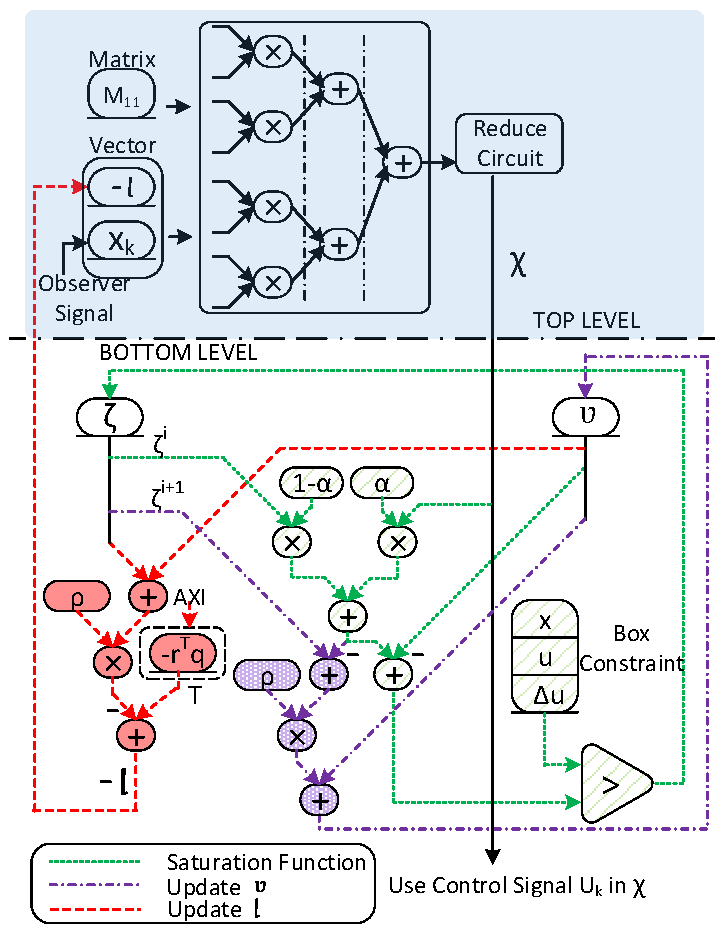
\includegraphics[scale=.40]{../ASAP_17/figure/architecture.pdf}
\DeclareGraphicsExtensions.
\caption{Hardware Architecture for ADMM with Relaxation Parameter $\alpha$.\label{fig_arch}}
\end{figure}
\end{columns}
\end{frame}
%------------------------------------------------
\begin{frame}
\frametitle{Hardware Architecture}
\framesubtitle{Reduce Circuit}
\begin{figure}[t]
\centering
\captionsetup{justification=centering}
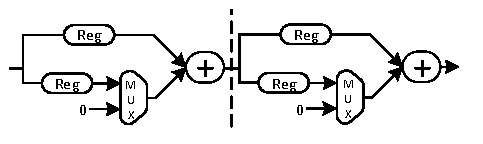
\includegraphics[scale=0.9]{../ASAP_17/figure/Reduce.pdf}
\DeclareGraphicsExtensions.
\caption{Reduce Circuit Architecture with Two Cascaded Adders\label{fig_red}}
\end{figure}
\end{frame}
%------------------------------------------------


\subsection{Trajectory Setting During Runtime}
%------------------------------------------------
\begin{frame}
\frametitle{Hardware Architecture}
\framesubtitle{Runtime Trajectory Planning}
\begin{figure}[t]
\centering
\captionsetup{justification=centering}
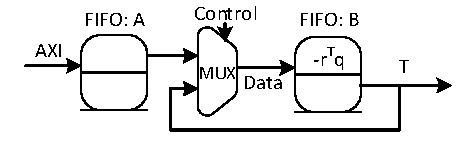
\includegraphics[scale=.75]{../ASAP_17/figure/trajectoryProfile.pdf}
\DeclareGraphicsExtensions.
\caption{Runtime Trajectory Planning\label{fig_traj}}
\end{figure}
\end{frame}

%------------------------------------------------

\subsection{Latency Analysis}
%------------------------------------------------
\begin{frame}

\end{frame}
%------------------------------------------------

\section{Evaluation}
%------------------------------------------------
\begin{frame}
\frametitle{Mass-spring System}
\end{frame}
%------------------------------------------------

%------------------------------------------------
\begin{frame}
\frametitle{Emulation using Plant on Chip}

\end{frame}
%------------------------------------------------

%------------------------------------------------
\begin{frame}
\frametitle{SW/HW Co-design}

\end{frame}
%------------------------------------------------

%------------------------------------------------
\begin{frame}
\frametitle{Computation Speed Versus Hardware Resources}

\end{frame}
%------------------------------------------------

%------------------------------------------------
\begin{frame}
\frametitle{Resource Utilization and Timing Summary}

\end{frame}
%------------------------------------------------



\section{Conclusion}



%------------------------------------------------

\begin{frame}
\frametitle{Bullet Points}
\begin{itemize}
\item Lorem ipsum dolor sit amet, consectetur adipiscing elit
\item Aliquam blandit faucibus nisi, sit amet dapibus enim tempus eu
\item Nulla commodo, erat quis gravida posuere, elit lacus lobortis est, quis porttitor odio mauris at libero
\item Nam cursus est eget velit posuere pellentesque
\item Vestibulum faucibus velit a augue condimentum quis convallis nulla gravida
\end{itemize}
\end{frame}

%------------------------------------------------

\begin{frame}
\frametitle{Blocks of Highlighted Text}
\begin{block}{Block 1}
Lorem ipsum dolor sit amet, consectetur adipiscing elit. Integer lectus nisl, ultricies in feugiat rutrum, porttitor sit amet augue. Aliquam ut tortor mauris. Sed volutpat ante purus, quis accumsan dolor.
\end{block}

\begin{block}{Block 2}
Pellentesque sed tellus purus. Class aptent taciti sociosqu ad litora torquent per conubia nostra, per inceptos himenaeos. Vestibulum quis magna at risus dictum tempor eu vitae velit.
\end{block}

\begin{block}{Block 3}
Suspendisse tincidunt sagittis gravida. Curabitur condimentum, enim sed venenatis rutrum, ipsum neque consectetur orci, sed blandit justo nisi ac lacus.
\end{block}
\end{frame}

%------------------------------------------------

\begin{frame}
\frametitle{Multiple Columns}
\begin{columns}[c] % The "c" option specifies centered vertical alignment while the "t" option is used for top vertical alignment

\column{.45\textwidth} % Left column and width
\textbf{Heading}
\begin{enumerate}
\item Statement
\item Explanation
\item Example
\end{enumerate}

\column{.5\textwidth} % Right column and width
Lorem ipsum dolor sit amet, consectetur adipiscing elit. Integer lectus nisl, ultricies in feugiat rutrum, porttitor sit amet augue. Aliquam ut tortor mauris. Sed volutpat ante purus, quis accumsan dolor.

\end{columns}
\end{frame}

%------------------------------------------------
\section{Second Section}
%------------------------------------------------

\begin{frame}
\frametitle{Table}
\begin{table}
\begin{tabular}{l l l}
\toprule
\textbf{Treatments} & \textbf{Response 1} & \textbf{Response 2}\\
\midrule
Treatment 1 & 0.0003262 & 0.562 \\
Treatment 2 & 0.0015681 & 0.910 \\
Treatment 3 & 0.0009271 & 0.296 \\
\bottomrule
\end{tabular}
\caption{Table caption}
\end{table}
\end{frame}

%------------------------------------------------

\begin{frame}
\frametitle{Theorem}
\begin{theorem}[Mass--energy equivalence]
$E = mc^2$
\end{theorem}
\end{frame}

%------------------------------------------------

\begin{frame}[fragile] % Need to use the fragile option when verbatim is used in the slide
\frametitle{Verbatim}
\begin{example}[Theorem Slide Code]
\begin{verbatim}
\begin{frame}
\frametitle{Theorem}
\begin{theorem}[Mass--energy equivalence]
$E = mc^2$
\end{theorem}
\end{frame}\end{verbatim}
\end{example}
\end{frame}

%------------------------------------------------

\begin{frame}
\frametitle{Figure}
Uncomment the code on this slide to include your own image from the same directory as the template .TeX file.
%\begin{figure}
%\includegraphics[width=0.8\linewidth]{test}
%\end{figure}
\end{frame}

%------------------------------------------------

\begin{frame}[fragile] % Need to use the fragile option when verbatim is used in the slide
\frametitle{Citation}
An example of the \verb|\cite| command to cite within the presentation:\\~

This statement requires citation \cite{p1}.
\end{frame}

%------------------------------------------------

\begin{frame}
\frametitle{References}
\footnotesize{
\begin{thebibliography}{99} % Beamer does not support BibTeX so references must be inserted manually as below
\bibitem[Smith, 2012]{p1} John Smith (2012)
\newblock Title of the publication
\newblock \emph{Journal Name} 12(3), 45 -- 678.
\end{thebibliography}
}
\end{frame}

%------------------------------------------------

\begin{frame}
\Huge{\centerline{The End}}
\end{frame}

%----------------------------------------------------------------------------------------

\end{document} 